\chapter{Input and output}

The programs we've looked at so far simply display messages, which doesn't involve a lot of real computation.
This chapter will show you how to read input from the keyboard, use that input to calculate a result, and then format that result for output.
%We will also look at some technical details about how operating systems work.


\section{The System class}
\label{sec:system}

\index{class!System}

We have been using \java{System.out.println} for a while, but you might not have thought about what it means.
\java{System} is a class that provides methods related to the ``system'' or environment where programs run.
It also provides \java{System.out}, which is a special value that provides methods for displaying output, including \java{println}.

\index{System.out}

In fact, we can use \java{System.out.println} to display the value of \java{System.out}:

\begin{code}
System.out.println(System.out);
\end{code}

The result is:

\begin{stdout}
java.io.PrintStream@685d72cd
\end{stdout}

\index{package}

This output indicates that \java{System.out} is a \java{PrintStream}, which is defined in a package called \java{java.io}.
A {\bf package} is a collection of related classes; \java{java.io} contains classes for ``I/O'' which stands for input and output.

\index{address}
\index{hexadecimal}

The numbers and letters after the {\tt @} sign are the {\bf address} of \java{System.out}, represented as a hexadecimal (base 16) number.
The address of a value is its location in the computer's memory, which might be different on different computers.
In this example the address is \java{685d72cd}, but if you run the same code you might get something different.
%You can think of the address as a unique identifier for the object.

\index{library}

As shown in Figure~\ref{fig.system}, \java{System} is defined in a file called {\tt System.java}, and \java{PrintStream} is defined in {\tt PrintStream.java}.
These files are part of the Java {\bf library}, which is an extensive collection of classes you can use in your programs.
%The source code for these classes is included with the JDK.

\begin{figure}[!ht]
\begin{center}
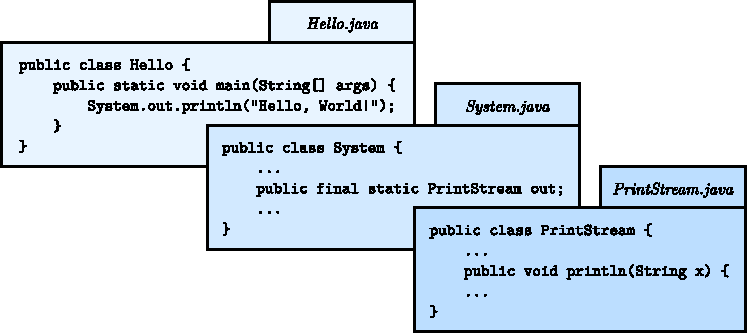
\includegraphics{figs/system.pdf}
\caption{\java{System.out.println} refers to the \java{out} variable of the \java{System} class, which is a \java{PrintStream} that provides a method called \java{println}.}
\label{fig.system}
\end{center}
\end{figure}


\section{The Scanner class}
\label{scanner}

\index{Scanner}
\index{class!Scanner}

%\index{byte}
%
%From the operating system's point of view, data from the keyboard arrives in a series of hardware control signals.
%The operating system translates these signals into a stream of {\bf bytes} (small integers), which in turn need to be translated into characters.
%\java{System.in} provides the means for reading one byte of input at a time, which is hardly useful for programs that would rather read in an entire word or line of input.

\index{System.in}

The \java{System} class also provides the special value \java{System.in}, which is an \java{InputStream} that provides methods for reading input from the keyboard.
These methods are not easy to use; fortunately, Java provides other classes that make it easier to handle common input tasks.

\index{class!utility}
\index{utility class}
\index{java.util}

For example, \java{Scanner} is a class that provides methods for inputting words, numbers, and other data.
\java{Scanner} is provided by \java{java.util}, which is a package that contains classes so useful they are called ``utility classes''.
Before you can use \java{Scanner}, you have to import it like this:

\begin{code}
import java.util.Scanner;
\end{code}

\index{import statement}
\index{statement!import}

This {\bf import statement} tells the compiler that when you say \java{Scanner}, you mean the one defined in \java{java.util}.
It's necessary because there might be another class named \java{Scanner} in another package.
Using an import statement makes your code unambiguous.

Import statements can't be inside a class definition.
By convention, they are usually at the beginning of the file.

Next you have to create a \java{Scanner}:

\begin{code}
Scanner in = new Scanner(System.in);
\end{code}

This line declares a \java{Scanner} variable named \java{in} and creates a new \java{Scanner} that takes input from \java{System.in}.
%We'll explain the \java{new} operator in more detail in Section~\ref{point}.

\java{Scanner} provides a method called \java{nextLine} that reads a line of input from the keyboard and returns a \java{String}.
The following example reads two lines and repeats them back to the user:

\begin{trinket}{Echo.java}
import java.util.Scanner;

public class Echo {

    public static void main(String[] args) {
        String line;
        Scanner in = new Scanner(System.in);

        System.out.print("Type something: ");
        line = in.nextLine();
        System.out.println("You said: " + line);

        System.out.print("Type something else: ");
        line = in.nextLine();
        System.out.println("You also said: " + line);
    }
}
\end{trinket}

If you omit the import statement and later refer to \java{Scanner}, you will get a compiler error like ``cannot find symbol''.
That means the compiler doesn't know what you mean by \java{Scanner}.

You might wonder why we can use the \java{System} class without importing it.
\java{System} belongs to the \java{java.lang} package, which is imported automatically.
According to the documentation, \java{java.lang} ``provides classes that are fundamental to the design of the Java programming language.''
The \java{String} class is also part of the \java{java.lang} package.


\section{Program structure}
\label{sec:library}

At this point, we have seen all of the elements that make up Java programs.
Figure~\ref{fig.package} shows these organizational units.

\begin{figure}[!ht]
\begin{center}
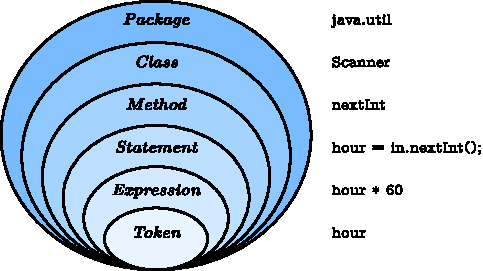
\includegraphics[width=4in]{figs/package.pdf}
\caption{Elements of the Java language, from largest to smallest.}
\label{fig.package}
\end{center}
\end{figure}

\index{token}

To review, a package is a collection of classes, which define methods.
Methods contain statements, some of which contain expressions.
Expressions are made up of {\bf tokens}, which are the basic elements of a program, including numbers, variable names, operators, keywords, and punctuation like parentheses, braces and semicolons.

The standard edition of Java comes with {\em several thousand} classes you can \java{import}, which can be both exciting and intimidating.
You can browse this library at \url{http://docs.oracle.com/javase/8/docs/api/}.
Most of the Java library itself is written in Java.

Note there is a major difference between the Java {\em language}, which defines the syntax and meaning of the elements in Figure~\ref{fig.package}, and the Java {\em library}, which provides the built-in classes.


\section{Inches to centimeters}

Now let's see an example that's a little more useful.
Although most of the world has adopted the metric system for weights and measures, some countries are stuck with English units.
For example, when talking with friends in Europe about the weather, people in the United States might have to convert from Celsius to Fahrenheit and back.
%And when making an international purchase online, you may have to convert your nation's currency into another based on the exchange rate.
Or they might want to convert height in inches to centimeters.

%An everyday problem that computers are great at solving is converting numbers from one unit into another.
%For the rest of the chapter, we will look at how to write programs that solve these types of problems.
%Specifically, each program will 1) prompt the user for input, 2) read input from the keyboard, 3) calculate a result, and 4) format the result for output.
%The focus will not only be on Java syntax and language features, but also on the {\em process} of solving the problem, documenting the code, and testing the solution.

We can write a program to help.
We'll use a \java{Scanner} to input a measurement in inches, convert to centimeters, and then display the results.
The following lines declare the variables and create the \java{Scanner}:

\begin{code}
int inch;
double cm;
Scanner in = new Scanner(System.in);
\end{code}

\index{nextInt!Scanner}

The next step is to prompt the user for the input.
We'll use \java{print} instead of \java{println} so they can enter the input on the same line as the prompt.
And we'll use the \java{Scanner} method \java{nextInt}, which reads input from the keyboard and converts it to an integer:

\begin{code}
System.out.print("How many inches? ");
inch = in.nextInt();
\end{code}

Next we multiply the number of inches by 2.54, since that's how many centimeters there are per inch, and display the results:

\begin{code}
cm = inch * 2.54;
System.out.print(inch + " in = ");
System.out.println(cm + " cm");
\end{code}

This code works correctly, but it has a minor problem.
If another programmer reads this code, they might wonder where 2.54 comes from.
For the benefit of others (and yourself in the future), it would be better to assign this value to a variable with a meaningful name.
We'll demonstrate in the next section.


\section{Literals and constants}

\index{literal}

A value that appears in a program, like 2.54 (or \java{" in ="}), is called a {\bf literal}.
In general, there's nothing wrong with literals.
But when numbers like 2.54 appear in an expression with no explanation, they make code hard to read.
And if the same value appears many times, and might have to change in the future, it makes code hard to maintain.

\index{magic number}

Values like that are sometimes called {\bf magic numbers} (with the implication that being ``magic'' is not a good thing).
A good practice is to assign magic numbers to variables with meaningful names, like this:

\begin{code}
double cmPerInch = 2.54;
cm = inch * cmPerInch;
\end{code}

This version is easier to read and less error-prone, but it still has a problem.
Variables can vary, but the number of centimeters in an inch does not.
Once we assign a value to \java{cmPerInch}, it should never change.
Java provides a language feature that enforces that rule, the keyword \java{final}.

\begin{code}
final double CM_PER_INCH = 2.54;
\end{code}

\index{final}
\index{constant}

Declaring that a variable is \java{final} means that it cannot be reassigned once it has been initialized.
If you try, the compiler reports an error.
Variables declared as \java{final} are called {\bf constants}.
By convention, names for constants are all uppercase, with the underscore character (\java{_}) between words.


\section{Formatting output}
\label{printf}

When you output a \java{double} using \java{print} or \java{println}, it displays up to 16 decimal places:

\begin{code}
System.out.print(4.0 / 3.0);
\end{code}

The result is:

\begin{stdout}
1.3333333333333333
\end{stdout}

\index{printf}

That might be more than you want.
\java{System.out} provides another method, called \java{printf}, that gives you more control of the format.
The ``f'' in \java{printf} stands for ``formatted''.
Here's an example:

\begin{code}
System.out.printf("Four thirds = %.3f", 4.0 / 3.0);
\end{code}

\index{format string}
\index{format specifier}

The first value in the parentheses is a {\bf format string} that specifies how the output should be displayed.
This format string contains ordinary text followed by a {\bf format specifier}, which is a special sequence that starts with a percent sign.
The format specifier \java{\%.3f} indicates that the following value should be displayed as floating-point, rounded to three decimal places.
The result is:

\begin{stdout}
Four thirds = 1.333
\end{stdout}

The format string can contain any number of format specifiers; here's an example with two:

\begin{code}
int inch = 100;
double cm = inch * CM_PER_INCH;
System.out.printf("%d in = %f cm\n", inch, cm);
\end{code}

The result is:

\begin{stdout}
100 in = 254.000000 cm
\end{stdout}

Like \java{print}, \java{printf} does not append a newline.
So format strings often end with a newline character.

The format specifier \java{\%d} displays integer values (``d'' stands for ``decimal'').
The values are matched up with the format specifiers in order, so \java{inch} is displayed using \java{\%d}, and \java{cm} is displayed using \java{\%f}.

Learning about format strings is like learning a sub-language within Java.
There are many options, and the details can be overwhelming.
Table~\ref{tab:format} lists a few common uses, to give you an idea of how things work.
For more details, refer to the documentation of \java{java.util.Formatter}.
The easiest way to find documentation for Java classes is to do a web search for ``Java'' and the name of the class.

\begin{table}[!ht]
\begin{center}
\begin{tabular}{|l|l|l|}
\hline
\java{\%d} & decimal integer & 12345 \\
\hline
%\java{\%,d} & decimal integer with comma separators & 12,345 \\
%\hline
\java{\%08d} & padded with zeros, at least 8 digits wide & 00012345 \\
\hline
\java{\%f} & floating-point & 6.789000 \\
\hline
\java{\%.2f} & rounded to 2 decimal places & 6.79 \\
\hline
\end{tabular}
\caption{Example format specifiers}
\label{tab:format}
\end{center}
\end{table}


\section{Centimeters to inches}
\label{sec:rounding}

Now suppose we have a measurement in centimeters, and we want to round it off to the nearest inch.
It is tempting to write:

\begin{code}
inch = cm / CM_PER_INCH;  // syntax error
\end{code}

But the result is an error -- you get something like, ``Bad types in assignment: from double to int.''
The problem is that the value on the right is floating-point, and the variable on the left is an integer.

%Java converts an \java{int} to a \java{double} automatically, since no information is lost in the process.
%On the other hand, going from \java{double} to \java{int} gets rid of the decimal places.
%Java doesn't perform this operation automatically in order to ensure that you are aware of the loss of the fractional part of the number.

\index{type cast}
\index{operator!cast}

The simplest way to convert a floating-point value to an integer is to use a {\bf type cast}, so called because it molds or ``casts'' a value from one type to another.
The syntax for type casting is to put the name of the type in parentheses and use it as an operator.

\begin{code}
double pi = 3.14159;
int x = (int) pi;
\end{code}

The \java{(int)} operator has the effect of converting what follows into an integer.
In this example, \java{x} gets the value \java{3}.
Like integer division, converting to an integer always rounds toward zero, even if the fraction part is \java{0.999999} (or \java{-0.999999}).
In other words, it simply throws away the fractional part.

Type casting takes precedence over arithmetic operations.
In this example, the value of \java{pi} gets converted to an integer before the multiplication.
So the result is 60.0, not 62.0.

\begin{code}
double pi = 3.14159;
double x = (int) pi * 20.0;
\end{code}

%Operator precedence and integer truncation make type casting somewhat error-prone.

Keeping that in mind, here's how we can convert a measurement in centimeters to inches:

\begin{code}
inch = (int) (cm / CM_PER_INCH);
System.out.printf("%f cm = %d in\n", cent, inch);
\end{code}

The parentheses after the cast operator require the division to happen before the type cast.
And the result is rounded toward zero; we will see in the next chapter how to round floating-point numbers to the closest integer.


%TODO replace modulus with modulo operation? or remainder operator?
\section{Modulus operator}

Let's take the example one step further: suppose you have a measurement in inches and you want to convert to feet and inches.
The goal is divide by 12 (the number of inches in a foot) and keep the remainder.

\index{modulus}
\index{\% operator}
\index{operator!modulus}

We have already seen the division operator (\java{/}), which computes the quotient of two numbers.
If the numbers are integers, it performs integer division.
Java also provides the {\bf modulus} operator (\java{\%}), which divides two numbers and computes the remainder.

Using division and modulus, we can convert to feet and inches like this:

\begin{code}
quotient = 76 / 12;   // division
remainder = 76 % 12;  // modulus
\end{code}

The first line yields 6.
The second line, which is pronounced ``76 mod 12'', yields 4.
So 76 inches is 6 feet, 4 inches.

The modulus operator looks like a percent sign, but you might find it helpful to think of it as a division sign ($\div$) rotated to the left.

%Note that both \java{/} and \java{\%} perform {\em integer division}, so the result always rounds down.
%The reason why integer division ``rounds down'' is that the hardware computes the quotient and remainder separately.

\index{divisible}
\index{extract digits}

The modulus operator turns out to be surprisingly useful.
For example, you can check whether one number is divisible by another: if \java{x \% y} is zero, then \java{x} is divisible by \java{y}.
You can use modulus to ``extract'' digits from a number: \java{x \% 10} yields the rightmost digit of \java{x}, and \java{x \% 100} yields the last two digits.
Also, many encryption algorithms use the modulus operator extensively.


\section{Putting it all together}

At this point, you have seen enough Java to write useful programs that solve everyday problems.
You can (1) import Java library classes, (2) create a \java{Scanner}, (3) get input from the keyboard, (4) format output with \java{printf}, and (5) divide and mod integers.
Now we will put everything together in a complete program:

%Since we've looked at each of these topics in isolation, it's important to see how they fit together in a complete program.
%If you've been working through the examples on your computer as you've been reading (like we recommended in Section~\ref{sec:examples}), then good job!

\begin{trinket}{Convert.java}
import java.util.Scanner;

/**
 * Converts centimeters to feet and inches.
 */
public class Convert {

    public static void main(String[] args) {
        double cm;
        int feet, inches, remainder;
        final double CM_PER_INCH = 2.54;
        final int IN_PER_FOOT = 12;
        Scanner in = new Scanner(System.in);

        // prompt the user and get the value
        System.out.print("Exactly how many cm? ");
        cm = in.nextDouble();

        // convert and output the result
        inches = (int) (cm / CM_PER_INCH);
        feet = inches / IN_PER_FOOT;
        remainder = inches % IN_PER_FOOT;
        System.out.printf("%.2f cm = %d ft, %d in\n",
                          cm, feet, remainder);
    }
}
\end{trinket}

Although not required, all variables and constants are declared at the top of \java{main}.
This practice makes it easier to find their types later on, and it helps the reader know what data is involved in the algorithm.

For readability, each major step of the algorithm is separated by a blank line and begins with a comment.
It also includes a documentation comment (\java{/**}), which we'll learn more about in the next chapter.

Many algorithms, including the \java{Convert} program, perform division and modulus together.
In both steps, you divide by the same number (\java{IN_PER_FOOT}).

When statements get long (generally wider than 80 characters), a common style convention is to break them across multiple lines.
The reader should never have to scroll horizontally.


\section{The Scanner bug}

Now that you've had some experience with \java{Scanner}, there is an unexpected behavior we want to warn you about.
The following code fragment asks users for their name and age:

\begin{code}
System.out.print("What is your name? ");
name = in.nextLine();
System.out.print("What is your age? ");
age = in.nextInt();
System.out.printf("Hello %s, age %d\n", name, age);
\end{code}

The output might look something like this:

\begin{stdout}
Hello Grace Hopper, age 45
\end{stdout}

When you read a \java{String} followed by an \java{int}, everything works just fine.
But when you read an \java{int} followed by a \java{String}, something strange happens.

\begin{code}
System.out.print("What is your age? ");
age = in.nextInt();
System.out.print("What is your name? ");
name = in.nextLine();
System.out.printf("Hello %s, age %d\n", name, age);
\end{code}

Try running this example code.
It doesn't let you input your name, and it immediately displays the output:

\begin{stdout}
What is your name? Hello , age 45
\end{stdout}

To understand what is happening, you have to understand that the \java{Scanner} doesn't see input as multiple lines, like we do.
Instead, it gets a ``stream of characters'' as shown in Figure~\ref{fig.hopper1}.

\begin{figure}[!ht]
\begin{center}
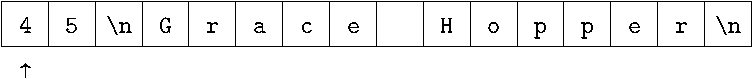
\includegraphics{figs/hopper1.pdf}
\caption{A stream of characters as seen by a \java{Scanner}.}
\label{fig.hopper1}
\end{center}
\end{figure}

The arrow indicates the next character to be read by \java{Scanner}.
When you call \java{nextInt}, it reads characters until it gets to a non-digit.
Figure~\ref{fig.hopper2} shows the state of the stream after \java{nextInt} is invoked.

\begin{figure}[!ht]
\begin{center}
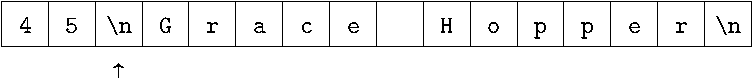
\includegraphics{figs/hopper2.pdf}
\caption{A stream of characters after \java{nextInt} is invoked.}
\label{fig.hopper2}
\end{center}
\end{figure}

At this point, \java{nextInt} returns \java{45}.
The program then displays the prompt \java{"What is your name? "} and calls \java{nextLine}, which reads characters until it gets to a newline.
But since the next character is already a newline, \java{nextLine} returns the empty string \java{""}.

To solve this problem, you need an extra \java{nextLine} after \java{nextInt}.

\begin{code}
System.out.print("What is your age? ");
age = in.nextInt();
in.nextLine();  // read the newline
System.out.print("What is your name? ");
name = in.nextLine();
System.out.printf("Hello %s, age %d\n", name, age);
\end{code}

This technique is common when reading \java{int} or \java{double} values that appear on their own line.
First you read the number, and then you read the rest of the line, which is just a newline character.


%TODO: DW suggests we also cover PrintWriter to write files
% add an appendix on File I/O since it involves try/catch?

\section{Vocabulary}

\begin{description}

\term{package}
A group of classes that are related to each other.
%Java classes are organized into packages.

\term{address}
The location of a value in computer memory, often represented as a hexadecimal integer.

\term{library}
A collection of packages and classes that are available for use in other programs.
%Libraries are often distributed in {\tt .jar} (Java Archive) files.

%\term{abstraction}
%The process of reducing information and/or detail to focus on high-level concepts.

%\term{operating system}
%Software that is always running behind the scenes on your computer.
%It controls the execution of application programs and manages hardware resources.

%\term{byte}
%A single unit of data on a computer; enough to represent one character.

%\term{utility class}
%A class that provides commonly needed functionality.

\term{import statement}
A statement that allows programs to use classes defined in other packages.

\term{token}
A basic element of a program, such as a word, space, symbol, or number.

\term{literal}
A value that appears in source code.
For example, \java{"Hello"} is a string literal and \java{74} is an integer literal.

\term{magic number}
A number that appears without explanation as part of an expression.
It should generally be replaced with a constant.

\term{constant}
A variable, declared \java{final}, whose value cannot be changed.

\term{format string}
A string passed to \java{printf} to specify the format of the output.

\term{format specifier}
A special code that begins with a percent sign and specifies the data type and format of the corresponding value.

\term{type cast}
An operation that explicitly converts one data type into another.
In Java it appears as a type name in parentheses, like \java{(int)}.

%\term{truncate}
%To make shorter by cutting something off.
%Casting a floating-point value to an integer simply removes the fractional part.

\term{modulus}
An operator that yields the remainder when one integer is divided by another.
In Java, it is denoted with a percent sign; for example, \java{5 \% 2} is \java{1}.

\end{description}


\section{Exercises}

The code for this chapter is in the {\tt ch03} directory of {\tt ThinkJavaCode}.
See page~\pageref{code} for instructions on how to download the repository.
Before you start the exercises, we recommend that you compile and run the examples.

If you have not already read Appendix~\ref{commandline}, now might be a good time.
It describes the command-line interface, which is a powerful and efficient way to interact with your computer.


\begin{exercise}
When you use \java{printf}, the Java compiler does not check your format string.
See what happens if you try to display a value with type \java{int} using \java{\%f}.
And what happens if you display a \java{double} using \java{\%d}?
What if you use two format specifiers, but then only provide one value?
\end{exercise}

%If you try to print an integer with \java{\%f} or a floating-point number using \java{\%d}, you get an \java{IllegalFormatConversionException}.


\begin{exercise}
Write a program that converts a temperature from Celsius to Fahrenheit.
It should (1) prompt the user for input, (2) read a \java{double} value from the keyboard, (3) calculate the result, and (4) format the output to one decimal place.
For example, it should display {\tt "24.0 C = 75.2 F"}.

Here is the formula.
Be careful not to use integer division!
%
\[ F = C \times \frac{9}{5} + 32 \]
\end{exercise}


\begin{exercise}
Write a program that converts a total number of seconds to hours, minutes, and seconds.
It should (1) prompt the user for input, (2) read an integer from the keyboard, (3) calculate the result, and (4) use \java{printf} to display the output.
For example, {\tt "5000 seconds = 1 hours, 23 minutes, and 20 seconds"}.

{\it Hint:} Use the modulus operator.
\end{exercise}


\begin{exercise}
\label{guess}
The goal of this exercise is to program a ``Guess My Number'' game.
When it's finished, it will work like this:

\begin{stdout}
I'm thinking of a number between 1 and 100
(including both). Can you guess what it is?
Type a number: 45
Your guess is: 45
The number I was thinking of is: 14
You were off by: 31
\end{stdout}

To choose a random number, you can use the \java{Random} class in \java{java.util}.
Here's how it works:

\begin{trinket}{GuessStarter.java}
import java.util.Random;

public class GuessStarter {

    public static void main(String[] args) {
        // pick a random number
        Random random = new Random();
        int number = random.nextInt(100) + 1;
        System.out.println(number);
    }
}
\end{trinket}

\index{new}
\index{operator!new}

Like the \java{Scanner} class we saw in this chapter, \java{Random} has to be imported before we can use it.
And as we saw with \java{Scanner}, we have to use the \java{new} operator to create a \java{Random} (number generator).

Then we can use the method \java{nextInt} to generate a random number.
In this example, the result of \java{nextInt(100)} will be between 0 and 99, including both.
Adding 1 yields a number between 1 and 100, including both.

\begin{enumerate}

\item The definition of \java{GuessStarter} is in a file called {\tt GuessStarter.java}, in the directory called {\tt ch03}, in the repository for this book.
%Instructions for downloading this code are on page~\pageref{code}.

\item Compile and run this program.

\item Modify the program to prompt the user, then use a \java{Scanner} to read a line of user input.
Compile and test the program.

\item Read the user input as an integer and display the result.
Again, compile and test.

\item Compute and display the difference between the user's guess and the number that was generated.

\end{enumerate}

\end{exercise}
